 % mainfile: ../../../../master.tex
\subsection{Troubleshoot DynDroid on AOSP 14}
\label{task:20240331_aosp}

\subsubsection{Integrate Changes to Zygote code}

Put customized code into remaining \path{dalvik_systemZygoteHooks.cc}, \path{odrefresh.cc}, and \path{odrefresh_main.cc}.

\subsubsection{Test Run Minima in Emulator}
Android is still crashing when using \texttt{adb install command}:
\begin{lstlisting}
adb install success_apps/53_com.technoskill.cricketscore.apk 
Performing Streamed Install
adb: failed to install success_apps/53_com.technoskill.cricketscore.apk: cmd: Failure calling service package: Broken pipe (32)
\end{lstlisting}

\subsubsection{Test Package Manager in AOSP14 Clean}

AOSP 14 Clean on P7Pro works for \texttt{adb install}.

Some have incompatible API versions: 
\begin{lstlisting}
adb install success_apps/68_im.dev.pregnancy.apk 
Performing Streamed Install
adb: failed to install success_apps/68_im.dev.pregnancy.apk: Failure [INSTALL_FAILED_DEPRECATED_SDK_VERSION: App package must target at least SDK version 23, but found 16]
\end{lstlisting}

\subsubsection{Preload Minima and Test Apps on Clean AOSP 14}
Cannot build anymore:
\begin{lstlisting}
internal error: bazel command failed: fork/exec ./build/bazel/bin/bazel: no such file or directory
\end{lstlisting}

Successfully preloaded \texttt{MedicalDrugDictionary.apk}, but the app crashes on load.

Deleted \texttt{out} directory, and successfully reran the \texttt{make} command.

Weird problem where \texttt{fastboot -w flashall} does not remove the apps from previous version of OS. So, just do \texttt{fastboot -w} and it'll wipe properly.

Somehow preloading APKs causes them to crash at load:
\begin{lstlisting}
03-31 15:04:36.501  4596  4596 W System.err: java.io.StreamCorruptedException: invalid stream header: 4DF493E3
03-31 15:04:36.501  4596  4596 W System.err: 	at java.io.ObjectInputStream.readStreamHeader(ObjectInputStream.java:865)
03-31 15:04:36.501  4596  4596 W System.err: 	at java.io.ObjectInputStream.<init>(ObjectInputStream.java:356)
03-31 15:04:36.501  4596  4596 W System.err: 	at com.atomic.apps.medical.drug.dictionary.a.b(Unknown Source:10)
03-31 15:04:36.501  4596  4596 W System.err: 	at com.atomic.apps.medical.drug.dictionary.a.c(Unknown Source:2)
03-31 15:04:36.502  4596  4596 W System.err: 	at com.atomic.apps.medical.drug.dictionary.a.b(Unknown Source:4)
03-31 15:04:36.502  4596  4596 W System.err: 	at com.atomic.apps.medical.drug.dictionary.a.<init>(Unknown Source:12)
03-31 15:04:36.502  4596  4596 W System.err: 	at com.atomic.apps.medical.drug.dictionary.a.a(Unknown Source:6)
03-31 15:04:36.502  4596  4596 W System.err: 	at com.atomic.apps.medical.drug.dictionary.DrugsListActivity.onCreate(Unknown Source:21)
03-31 15:04:36.502  4596  4596 W System.err: 	at android.app.Activity.performCreate(Activity.java:8621)
03-31 15:04:36.502  4596  4596 W System.err: 	at android.app.Activity.performCreate(Activity.java:8599)
03-31 15:04:36.502  4596  4596 W System.err: 	at android.app.Instrumentation.callActivityOnCreate(Instrumentation.java:1456)
03-31 15:04:36.502  4596  4596 W System.err: 	at android.app.ActivityThread.performLaunchActivity(ActivityThread.java:3804)
03-31 15:04:36.502  4596  4596 W System.err: 	at android.app.ActivityThread.handleLaunchActivity(ActivityThread.java:3963)
03-31 15:04:36.502  4596  4596 W System.err: 	at android.app.servertransaction.LaunchActivityItem.execute(LaunchActivityItem.java:103)
03-31 15:04:36.502  4596  4596 W System.err: 	at android.app.servertransaction.TransactionExecutor.executeCallbacks(TransactionExecutor.java:139)
03-31 15:04:36.502  4596  4596 W System.err: 	at android.app.servertransaction.TransactionExecutor.execute(TransactionExecutor.java:96)
03-31 15:04:36.502  4596  4596 W System.err: 	at android.app.ActivityThread$H.handleMessage(ActivityThread.java:2468)
03-31 15:04:36.502  4596  4596 W System.err: 	at android.os.Handler.dispatchMessage(Handler.java:106)
03-31 15:04:36.502  4596  4596 W System.err: 	at android.os.Looper.loopOnce(Looper.java:205)
03-31 15:04:36.502  4596  4596 W System.err: 	at android.os.Looper.loop(Looper.java:294)
03-31 15:04:36.502  4596  4596 W System.err: 	at android.app.ActivityThread.main(ActivityThread.java:8248)
03-31 15:04:36.502  4596  4596 W System.err: 	at java.lang.reflect.Method.invoke(Native Method)
03-31 15:04:36.502  4596  4596 W System.err: 	at com.android.internal.os.RuntimeInit$MethodAndArgsCaller.run(RuntimeInit.java:552)
03-31 15:04:36.502  4596  4596 W System.err: 	at com.android.internal.os.ZygoteInit.main(ZygoteInit.java:971)
03-31 15:04:36.502  4596  4596 W System.err: java.io.StreamCorruptedException: invalid stream header: 35BBE049
03-31 15:04:36.502  4596  4596 W System.err: 	at java.io.ObjectInputStream.readStreamHeader(ObjectInputStream.java:865)
03-31 15:04:36.502  4596  4596 W System.err: 	at java.io.ObjectInputStream.<init>(ObjectInputStream.java:356)
03-31 15:04:36.502  4596  4596 W System.err: 	at com.atomic.apps.medical.drug.dictionary.a.b(Unknown Source:10)
03-31 15:04:36.502  4596  4596 W System.err: 	at com.atomic.apps.medical.drug.dictionary.a.c(Unknown Source:10)
03-31 15:04:36.502  4596  4596 W System.err: 	at com.atomic.apps.medical.drug.dictionary.a.b(Unknown Source:4)
03-31 15:04:36.502  4596  4596 W System.err: 	at com.atomic.apps.medical.drug.dictionary.a.<init>(Unknown Source:12)
03-31 15:04:36.502  4596  4596 W System.err: 	at com.atomic.apps.medical.drug.dictionary.a.a(Unknown Source:6)
03-31 15:04:36.502  4596  4596 W System.err: 	at com.atomic.apps.medical.drug.dictionary.DrugsListActivity.onCreate(Unknown Source:21)
03-31 15:04:36.502  4596  4596 W System.err: 	at android.app.Activity.performCreate(Activity.java:8621)
03-31 15:04:36.502  4596  4596 W System.err: 	at android.app.Activity.performCreate(Activity.java:8599)
03-31 15:04:36.502  4596  4596 W System.err: 	at android.app.Instrumentation.callActivityOnCreate(Instrumentation.java:1456)
03-31 15:04:36.502  4596  4596 W System.err: 	at android.app.ActivityThread.performLaunchActivity(ActivityThread.java:3804)
03-31 15:04:36.502  4596  4596 W System.err: 	at android.app.ActivityThread.handleLaunchActivity(ActivityThread.java:3963)
03-31 15:04:36.502  4596  4596 W System.err: 	at android.app.servertransaction.LaunchActivityItem.execute(LaunchActivityItem.java:103)
03-31 15:04:36.502  4596  4596 W System.err: 	at android.app.servertransaction.TransactionExecutor.executeCallbacks(TransactionExecutor.java:139)
03-31 15:04:36.502  4596  4596 W System.err: 	at android.app.servertransaction.TransactionExecutor.execute(TransactionExecutor.java:96)
03-31 15:04:36.502  4596  4596 W System.err: 	at android.app.ActivityThread$H.handleMessage(ActivityThread.java:2468)
03-31 15:04:36.502  4596  4596 W System.err: 	at android.os.Handler.dispatchMessage(Handler.java:106)
03-31 15:04:36.502  4596  4596 W System.err: 	at android.os.Looper.loopOnce(Looper.java:205)
03-31 15:04:36.502  4596  4596 W System.err: 	at android.os.Looper.loop(Looper.java:294)
03-31 15:04:36.502  4596  4596 W System.err: 	at android.app.ActivityThread.main(ActivityThread.java:8248)
03-31 15:04:36.502  4596  4596 W System.err: 	at java.lang.reflect.Method.invoke(Native Method)
03-31 15:04:36.502  4596  4596 W System.err: 	at com.android.internal.os.RuntimeInit$MethodAndArgsCaller.run(RuntimeInit.java:552)
03-31 15:04:36.502  4596  4596 W System.err: 	at com.android.internal.os.ZygoteInit.main(ZygoteInit.java:971)
03-31 15:04:36.502  4596  4596 D com.atomic.apps.medical.drug.dictionary: Using B
03-31 15:04:36.502  4596  4596 D AndroidRuntime: Shutting down VM
03-31 15:04:36.502  4596  4596 E AndroidRuntime: FATAL EXCEPTION: main
03-31 15:04:36.502  4596  4596 E AndroidRuntime: Process: com.atomic.apps.medical.drug.dictionary, PID: 4596
03-31 15:04:36.502  4596  4596 E AndroidRuntime: java.lang.RuntimeException: Unable to start activity ComponentInfo{com.atomic.apps.medical.drug.dictionary/com.atomic.apps.medical.drug.dictionary.DrugsListActivity}: java.lang.NullPointerException: Attempt to invoke virtual method 'byte[] java.lang.String.getBytes()' on a null object reference
03-31 15:04:36.502  4596  4596 E AndroidRuntime: 	at android.app.ActivityThread.performLaunchActivity(ActivityThread.java:3822)
03-31 15:04:36.502  4596  4596 E AndroidRuntime: 	at android.app.ActivityThread.handleLaunchActivity(ActivityThread.java:3963)
03-31 15:04:36.502  4596  4596 E AndroidRuntime: 	at android.app.servertransaction.LaunchActivityItem.execute(LaunchActivityItem.java:103)
03-31 15:04:36.502  4596  4596 E AndroidRuntime: 	at android.app.servertransaction.TransactionExecutor.executeCallbacks(TransactionExecutor.java:139)
03-31 15:04:36.502  4596  4596 E AndroidRuntime: 	at android.app.servertransaction.TransactionExecutor.execute(TransactionExecutor.java:96)
03-31 15:04:36.502  4596  4596 E AndroidRuntime: 	at android.app.ActivityThread$H.handleMessage(ActivityThread.java:2468)
03-31 15:04:36.502  4596  4596 E AndroidRuntime: 	at android.os.Handler.dispatchMessage(Handler.java:106)
03-31 15:04:36.502  4596  4596 E AndroidRuntime: 	at android.os.Looper.loopOnce(Looper.java:205)
03-31 15:04:36.502  4596  4596 E AndroidRuntime: 	at android.os.Looper.loop(Looper.java:294)
03-31 15:04:36.502  4596  4596 E AndroidRuntime: 	at android.app.ActivityThread.main(ActivityThread.java:8248)
03-31 15:04:36.502  4596  4596 E AndroidRuntime: 	at java.lang.reflect.Method.invoke(Native Method)
03-31 15:04:36.502  4596  4596 E AndroidRuntime: 	at com.android.internal.os.RuntimeInit$MethodAndArgsCaller.run(RuntimeInit.java:552)
03-31 15:04:36.502  4596  4596 E AndroidRuntime: 	at com.android.internal.os.ZygoteInit.main(ZygoteInit.java:971)
03-31 15:04:36.502  4596  4596 E AndroidRuntime: Caused by: java.lang.NullPointerException: Attempt to invoke virtual method 'byte[] java.lang.String.getBytes()' on a null object reference
03-31 15:04:36.502  4596  4596 E AndroidRuntime: 	at com.atomic.apps.medical.drug.dictionary.a.a(Unknown Source:0)
03-31 15:04:36.502  4596  4596 E AndroidRuntime: 	at com.atomic.apps.medical.drug.dictionary.a.b(Unknown Source:8)
03-31 15:04:36.502  4596  4596 E AndroidRuntime: 	at com.atomic.apps.medical.drug.dictionary.a.<init>(Unknown Source:12)
03-31 15:04:36.502  4596  4596 E AndroidRuntime: 	at com.atomic.apps.medical.drug.dictionary.a.a(Unknown Source:6)
03-31 15:04:36.502  4596  4596 E AndroidRuntime: 	at com.atomic.apps.medical.drug.dictionary.DrugsListActivity.onCreate(Unknown Source:21)
03-31 15:04:36.502  4596  4596 E AndroidRuntime: 	at android.app.Activity.performCreate(Activity.java:8621)
03-31 15:04:36.502  4596  4596 E AndroidRuntime: 	at android.app.Activity.performCreate(Activity.java:8599)
03-31 15:04:36.502  4596  4596 E AndroidRuntime: 	at android.app.Instrumentation.callActivityOnCreate(Instrumentation.java:1456)
03-31 15:04:36.502  4596  4596 E AndroidRuntime: 	at android.app.ActivityThread.performLaunchActivity(ActivityThread.java:3804)
03-31 15:04:36.502  4596  4596 E AndroidRuntime: 	... 12 more
03-31 15:04:36.504  1496  2267 W ActivityTaskManager:   Force finishing activity com.atomic.apps.medical.drug.dictionary/.DrugsListActivity
\end{lstlisting}

\subsubsection{Replace Framework and Run}

\texttt{PackageManager.java}, \texttt{DefaultPermissionGrantPolicy.java}, \texttt{PermissionManagerServiceImpl.java}, \texttt{ParsingPackageUtils.java} has only trivial logging code. 

\texttt{PermissionManagerService.java} has some changes to requested permissions in \texttt{onPackageInstalled}. \texttt{PackageParser.java} has changes to \texttt{parseBaseApkCommon}.

Same problem with emulator version:
\begin{lstlisting}
adb install success_apps/60_com.atomic.apps.medical.drug.dictionary.apk 
Performing Streamed Install
adb: failed to install success_apps/60_com.atomic.apps.medical.drug.dictionary.apk: cmd: Failure calling service package: Broken pipe (32)    
\end{lstlisting}

Logcat output:
\begin{lstlisting}
03-31 15:47:11.367  6659  6709 E AndroidRuntime: *** FATAL EXCEPTION IN SYSTEM PROCESS: PackageManager
03-31 15:47:11.367  6659  6709 E AndroidRuntime: java.lang.UnsupportedOperationException
03-31 15:47:11.367  6659  6709 E AndroidRuntime: 	at java.util.Collections$UnmodifiableCollection.add(Collections.java:1114)
03-31 15:47:11.367  6659  6709 E AndroidRuntime: 	at com.android.server.pm.permission.PermissionManagerService$PermissionManagerServiceInternalImpl.onPackageInstalled(PermissionManagerService.java:706)
03-31 15:47:11.367  6659  6709 E AndroidRuntime: 	at com.android.server.pm.InstallPackageHelper.updateSettingsInternalLI(InstallPackageHelper.java:2370)
03-31 15:47:11.367  6659  6709 E AndroidRuntime: 	at com.android.server.pm.InstallPackageHelper.updateSettingsLI(InstallPackageHelper.java:2165)
03-31 15:47:11.367  6659  6709 E AndroidRuntime: 	at com.android.server.pm.InstallPackageHelper.commitPackagesLocked(InstallPackageHelper.java:2134)
03-31 15:47:11.367  6659  6709 E AndroidRuntime: 	at com.android.server.pm.InstallPackageHelper.installPackagesLI(InstallPackageHelper.java:1031)
03-31 15:47:11.367  6659  6709 E AndroidRuntime: 	at com.android.server.pm.InstallPackageHelper.installPackagesTraced(InstallPackageHelper.java:915)
03-31 15:47:11.367  6659  6709 E AndroidRuntime: 	at com.android.server.pm.InstallingSession.processApkInstallRequests(InstallingSession.java:540)
03-31 15:47:11.367  6659  6709 E AndroidRuntime: 	at com.android.server.pm.InstallingSession.processInstallRequests(InstallingSession.java:529)
03-31 15:47:11.367  6659  6709 E AndroidRuntime: 	at com.android.server.pm.InstallingSession.lambda$processPendingInstall$0(InstallingSession.java:288)
03-31 15:47:11.367  6659  6709 E AndroidRuntime: 	at com.android.server.pm.InstallingSession.$r8$lambda$tqRjKCgCJYNNnnY7Qw5M5BHLup8(InstallingSession.java:0)
03-31 15:47:11.367  6659  6709 E AndroidRuntime: 	at com.android.server.pm.InstallingSession$$ExternalSyntheticLambda1.run(R8$$SyntheticClass:0)
03-31 15:47:11.367  6659  6709 E AndroidRuntime: 	at android.os.Handler.handleCallback(Handler.java:958)
03-31 15:47:11.367  6659  6709 E AndroidRuntime: 	at android.os.Handler.dispatchMessage(Handler.java:99)
03-31 15:47:11.367  6659  6709 E AndroidRuntime: 	at android.os.Looper.loopOnce(Looper.java:205)
03-31 15:47:11.367  6659  6709 E AndroidRuntime: 	at android.os.Looper.loop(Looper.java:294)
03-31 15:47:11.367  6659  6709 E AndroidRuntime: 	at android.os.HandlerThread.run(HandlerThread.java:67)
03-31 15:47:11.367  6659  6709 E AndroidRuntime: 	at com.android.server.ServiceThread.run(ServiceThread.java:46)  
\end{lstlisting}

Problematic code:
\begin{lstlisting}      
String name = "edu.smu.minimaconfig.MyContentProvider.READ";
int index_1 = pkg.getRequestedPermissions().indexOf(name);
if (index_1 == -1) {
    pkg.getRequestedPermissions().add(name.intern());
    Slog.w("zicheng_framework", "[Zicheng_frameworks]onPackageInstalled() add permission:"
            + name + " in package: " + pkg.getPackageName());
} else {
    Slog.w("zicheng_framework", "[Zicheng_frameworks]onPackageInstalled() Ignoring duplicate uses-permissions/uses-permissions-sdk-m: "
            + name + " in package: " + pkg.getPackageName());
}
if(pkg.getRequestedPermissions().size()>0)
    for(int kk=0;kk<pkg.getRequestedPermissions().size();kk++)
        Slog.w("zicheng_framework", "[Zicheng_frameworks]PermissionManagerService.java onPackageInstalled()"+
                " in package: " + pkg.getPackageName() + "permission num: "+kk+":"+pkg.getRequestedPermissions().get(kk));
\end{lstlisting}
Removed this line of code from emulator project also. The app can be successfully \texttt{adb install}ed but the app crashes after loading splash screen for a long time.

% 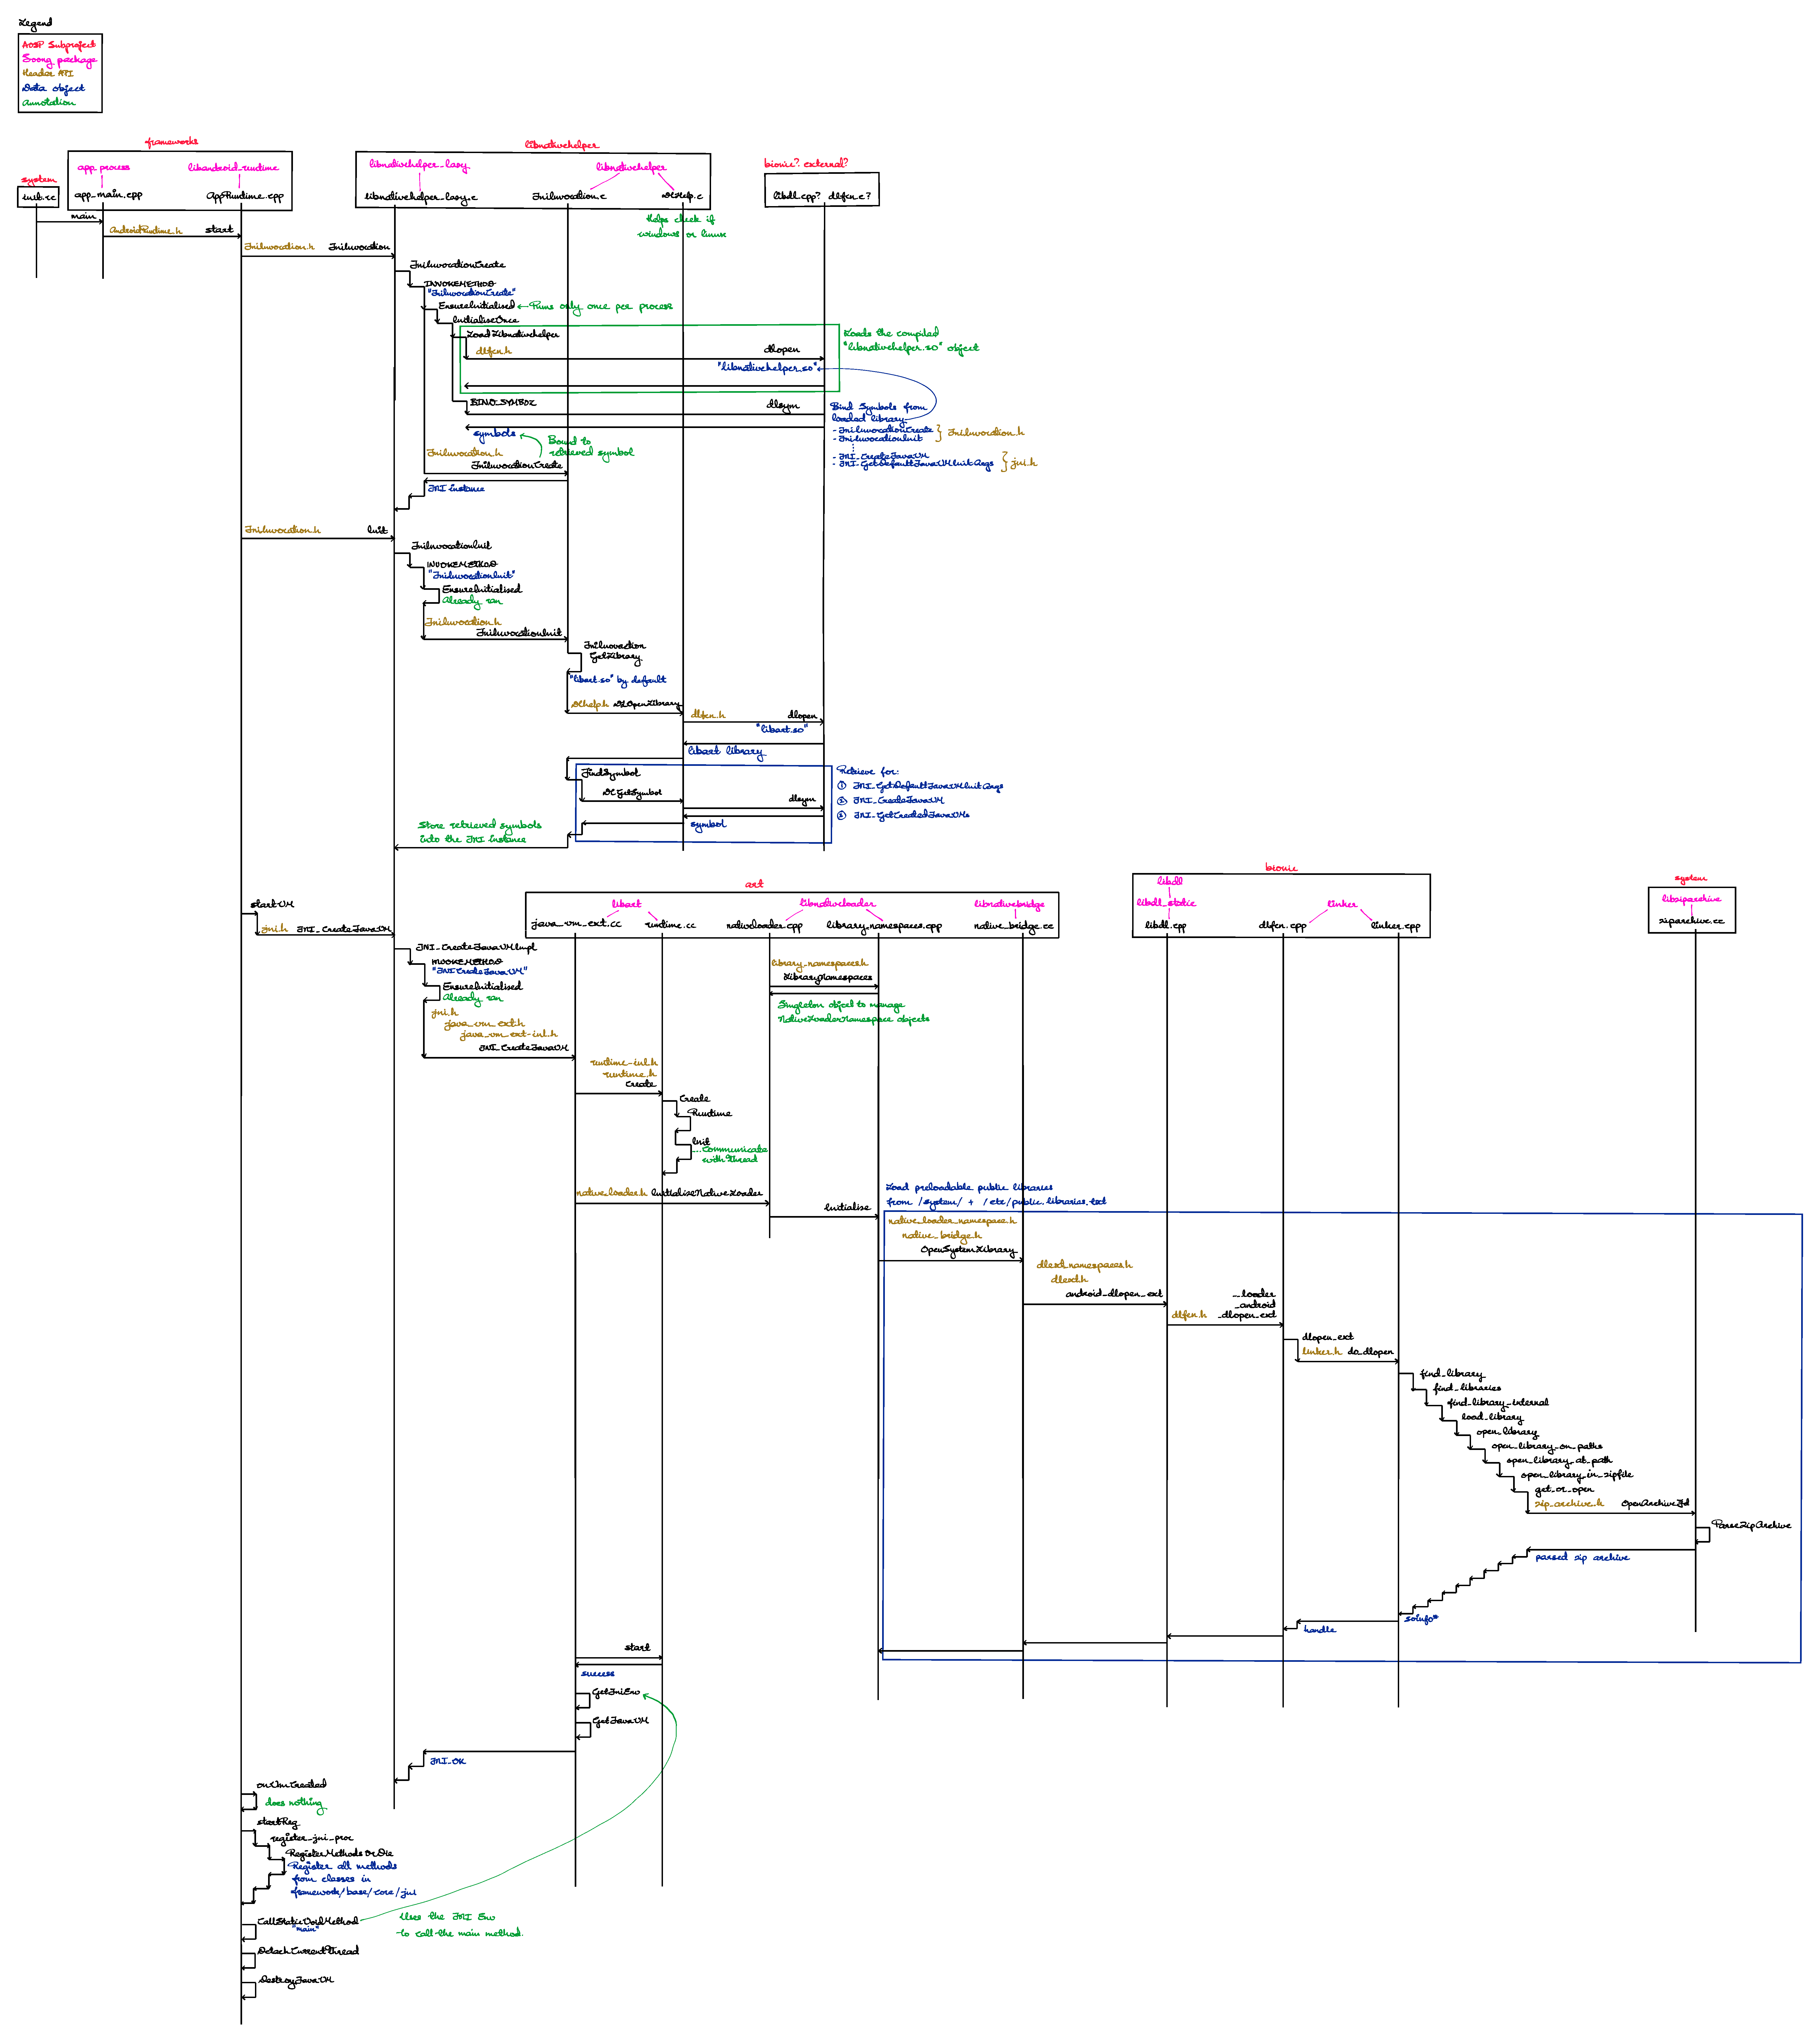
\includepdf[pages=-, scale=.95,pagecommand={}]{entries/2024/01/01/art.pdf}

% \begin{itemize}
% \item \textbf{Domain.} The context of the process that is acting upon something.
% \item \textbf{Type.} The context of the resource on which the process is acting.
% \item \textbf{Class.} The object class of the resource (e.g. \textit{file} or \textit{socket}).
% \item \textbf{Permissions.} The permissions that are allowed given the \textit{domain}, \textit{type} and \textit{class}.
% \end{itemize}

% SELinux rule syntax:


% \subsubsection{Decoding Permission Denial Message}

% Message:
% \begin{lstlisting}
% type=AVC msg=audit(1363289005.532:184): avc:  denied  { read } for  pid=29199 comm="Trace" 
% name="online" dev="sysfs" ino=30 scontext=staff_u:staff_r:googletalk_plugin_t 
% tcontext=system_u:object_r:sysfs_t tclass=file
% \end{lstlisting}

% \begin{longtable}{p{.15\linewidth}p{.15\linewidth}p{.65\linewidth}} 
% \toprule
% Log part & Name & Description \\
% \midrule
% \endhead

% \texttt{type=AVC}
% &Log type
% &Only in the \texttt{audit.log} file; it informs the user what kind of audit log type this is. 
% \\

% \texttt{msg=audit(1363289005.532:184)}
% &Timestamp
% &Timestamp in seconds since epoch, meaning the number of seconds since January 1st, 1970. You can convert this to a more human readable format using date -d @ followed by the number, like so: \texttt{date -d @1363292159.532}.
% \\

% \texttt{avc:}
% &Log type (again)
% &
% \\

% \texttt{ino=30}
% &inode number
% &The inode number of the target file. In this case, since we know it is on the \texttt{sysfs} file system, we can look for this file using: \texttt{find /sys -xdev -inum 30}
% \\

% \texttt{scontent=staff\_u:staff\_r:googletalk\_plugin\_t}
% &Source context
% &The security context of the process (the domain)
% \\

% \texttt{tcontext=system\_u:object\_r:sysfs\_t}
% &Target context
% &The security context of the target resource (in this case the file)
% \\

% \texttt{tclass=file}
% &Target class
% &The class of the target.
% \\

% \midrule
% \caption{Permission Denied Syntax} 
% \label{tab:permissiondeniedsyntax}
% \end{longtable}


% \subsubsection{SELinux Architecture}

% SELinux consists of four main components: object managers (OM), access vector cache (AVC), security server, and security policy as show below:
% \begin{figure}[H]
%     \centering
%     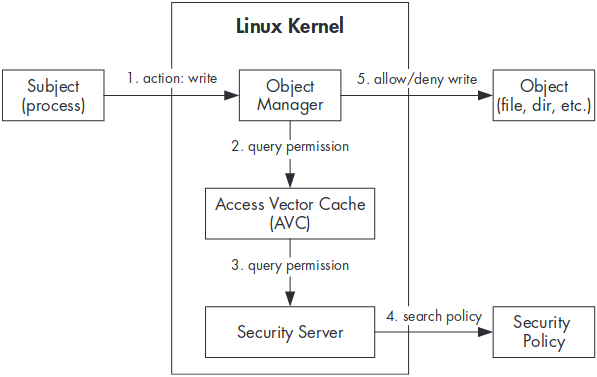
\includegraphics[width=.85\linewidth]{entries/2023/12/10/selinux.png}
%     \caption{SELinux Components}
%     \label{fig:selinux}
% \end{figure}
